%!TEX root = ../main.tex

\section{Strongly Connected Components}

Suppose $G = (V, E)$ is a directed graph. What is the correct connectivity
relation in a directed graph? Define a relation $R = \{ (u, v) :
\text{there is a path from $u$ to $v$ and from $v$ to $u$} \}$. Note
we bake into the definition symmetry. For instance, for the graph
$1 \to 2$, we have that $R = \{ (1, 1), (2, 2) \}$. This relation is
in fact an equivalence relation (exercise: show it). We know then
that $R$ partitions $V$ into equivalence classes $V_1, V_2, ..., V_k$.

\begin{definition}
    For any $i = 1 \to k$, we have that 
    $G_i = (V_i, E \cap V_i \times V_i)$ is a strongly 
    connected component of $G$.
\end{definition}

Note that you
could have an edge connecting $G_i$ and $G_j$. Let each $G_i$ denote a
vertex in a new graph $G_{SCC}$. This is the
strongly connected component graph of $G$. More formally,
we have that $G_{SCC} = (V_{SCC}, E_{SCC})$ where 
$V_{SCC} = \{ C_i : C_i \text{is a strongly connected component} \}$
and $E_{SCC} = \{ (c_i, c_j) : \text{there exists
$v_i \in C_i$ and $v_j \in C_j$ such that $(v_i, v_j) \in E$} \}$. For
an example, take a look at Figure~\ref{fig:scc}.

\begin{figure}[hpt]
    \centering
    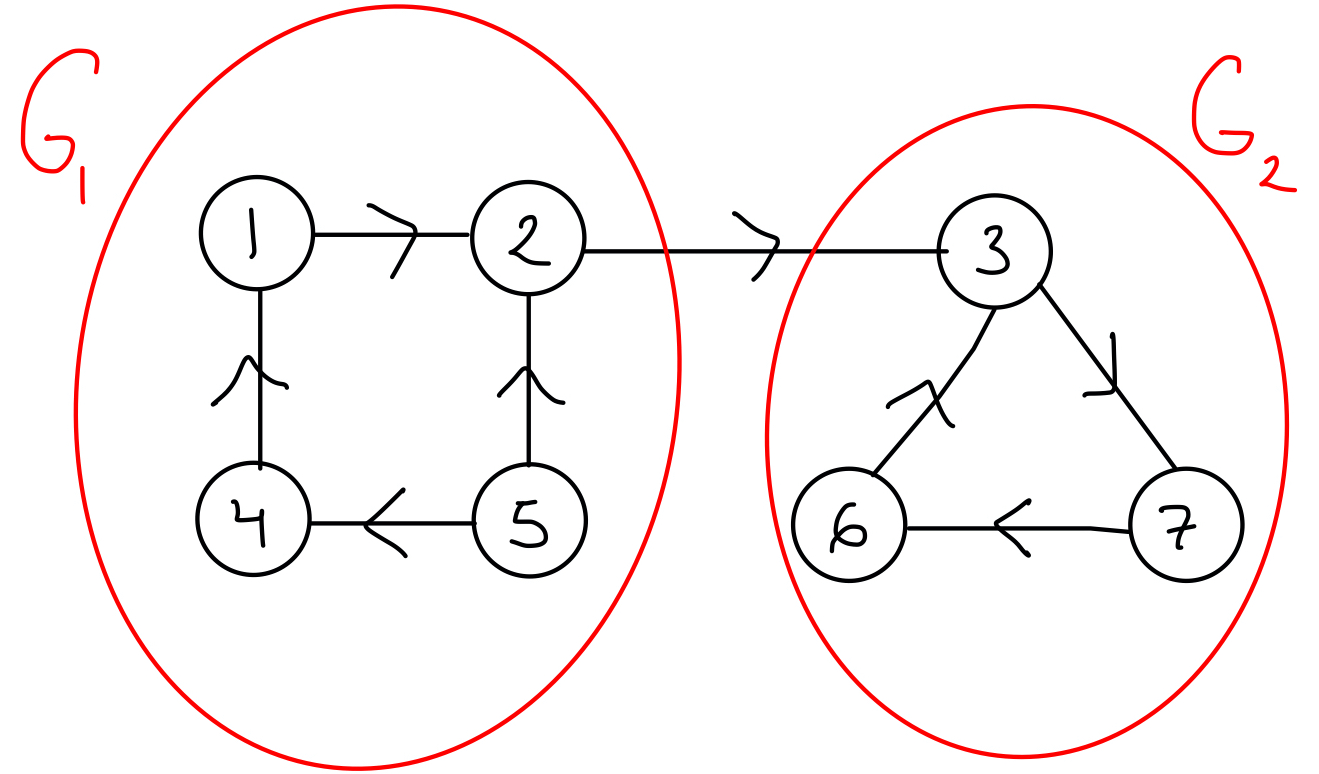
\includegraphics[width=0.45\textwidth]{figures/scc.jpeg}
    \caption{Example of a graph with strongly connected components.
    The
    equivalence classes are $\{\{1, 2, 4, 5 \},  \{3, 6, 7\}\}$. The
    $G_{SCC}$ is simply $C_1 \to C_2$.}
    \label{fig:scc}
\end{figure}

\begin{lemma}
    $G_{SCC}$ is acyclic.
\end{lemma}

DFS will decompose a directed graph $G$ into its SCC. Let $G$ be an
arbitrary directed graph. We know $G_{SCC}$ is a DAG by the above
lemma.

\begin{lemma}
    (False lemma!) If $C_1$ and $C_2$ are SCC and $(C_1, C_2) \in E_
    {SCC}$ then
    in a DFS of $G$, every vertex in $G_1$ finishes after every vertex
    in $G_2$.
\end{lemma}

Why is this wrong? Look at Figure~\ref{fig:scc} and figure it out.

\begin{lemma}
    (Correct lemma) If $C_1$ and $C_2$ are SCC and $(C_1, C_2) \in E_
    {SCC}$ then
    in a DFS of $G$, there exists a vertex in $G_1$ that finishes
    after every vertex
    in $G_2$.
\end{lemma}

\begin{proof}
    Look at the book.
\end{proof}

Let's recapitulate.

\begin{itemize}
    \item We know $G_{SCC}$ is a DAG.
    \item $G_{SCC}$ has one or more vertices with no incoming edges.
    These vertices are called sources. Therefore, if $v$ has the
    largest finishing time $f(v)$ in a DFS of $G$, then $v$ must lie
    in a source component.
\end{itemize}

\subsubsection{Kosaraju's Algorithm}

(Very informal, for more info visit 
\href{https://en.wikipedia.org/wiki/Kosaraju%27s_algorithm}{here}). Perform one DFS to record the
order of finishing times. Let $f_1(v)$ be the finish time of $v$ in this DFS.
Now reverse all the edges in $G$ to create the graph $G^R$ and perform a second DFS of $G^R$ with one constraint: In the outer procedure always choose the undiscovered vertex $v$ with greatest $f_1(v)$ (note that the vertex $v$ with greatest $f_1(v)$ lies in a sink component in $G^R$).
We know $G$ and $G^R$ have the same strongly connected components. We also
know that, since $v$ is in a sink component, the DFS of $G^R$ started at $v$
will only discover the SCC containing $v$. When the inner call to 
DFS($G^R, v$) finishes, output all the discovered vertices as one SCC of $G$.
When we return to the outer loop and pick the undiscovered vertex with
greatest finish time, we know inductively that we will find all SCCs.
The running time of the algorithm is the time it takes to performs two
DFS, which is $O(n)$.

\section{Optimization}

In this type of problems, we would like to minimize/maximize some
function subject to some constraints. A special class of optimizations
problems is the following: Given a set of elements, pick a subset,
where the constraints tell you which subsets are allowed (we call
them \textbf{feasible} solutions). We will have an objective
function that assigns a value to every feasible solution.

\subsection{Minimum Spanning Tree}

The input to this problem is an undirected, connected graph $G = (V,
E)$ together with weights on the edges, where $w: E \to \mathbb{R}^+$.
A feasible solution will be a set of edges that form an acyclic,
connected graph on all vertices. The cost of a solution is the sum of
the weights of the edges in the solution.

\section{Greedy Algorithms}

There are problems for which
the optimum solution can be chosen by choosing one element at a time.
We can solve this problems with greedy algorithms.

\begin{definition}
    A greedy algorithm builds up a solution $S$ by taking at each
    turn the next element with optimal cost that can be added
    feasibly.
\end{definition}

\subsection{Activity Selection Problem}

This is a classic problem that can be solved using a greedy algorithm.
The input is $n$ activities, where $a_i = (s_i, f_i)$ starts at time
$s_i$ and finishes at time $f_i$. A feasible solution will be any
subset of these activities such that no two activities overlap. The
optimization problem will be to maximize the number of activities
scheduled.

Let's propose some criteria to be greedy on.

\begin{itemize}
    \item Pick the activity with shortest duration. This won't work,
    because if you have long activities $n_1 = (1, 10)$ and $n_2 = 
    (11,
    20)$ and a short activity $n_3 = (9, 12)$, this approach will
    only pick $n_3$ with a value of 1 while an optimal solution will
    have a value of 2 (by choosing $n_1$ and $n_2$).
    \item  Pick the activity that finishes first. Sort the activities
    by finish time and reorder them as $a_1, a_2, ..., a_n$ so that
    $f_1 \leq f_2, ... \leq f_n$. Now pick $a_1$ and remove all
    activities that have a conflict with $a_1$, and repeat this
    process.
\end{itemize}

The second approach is correct, but can we prove this? 

\begin{definition}
    The greedy choice property states that the
first choice made by a greedy algorithm is not wrong.
\end{definition}

In this case, the greedy choice property means that if we
choose $a_1$ first, then there is an optimal
feasible solution that contains $a_1$. Suppose for a contradiction
that no optimal solution uses $a_1$. Let $O$ be the subset of
activities in some optimal solution. We can order the activities in
$O$ by finish time. Let $a_{i_1}, ..., a_{i_k}$ be this ordering.
We claim that we can throw away $a_{i_1}$ and replace it with $a_1$.
This is called the \textbf{exchange} argument. We now have $O' = O -
\{a_{i_1}\} \cup \{a_1\}$. But by our greedy assumption the finish
time of $a_1$ is less than the finish time of $a_{i_1}$, so $a_1$
doesn't overlap with $a_{i_2}$ and $O'$ is an optimal solution, which
is a contradiction.

We've just shown there is an optimal solution that starts with $a_1$.
This optimal solution should certainly exclude activities that have a
conflict with $a_1$. Recursively, we need to solve a smaller problem
consisting of activities that don't conflict with $a_1$. In this set
of activities, we need to pick an optimal, feasible subset. 

Let $A$ be the original set of activities, and let $A'$ be the
remaining set of activities after throwing out $a_1$ and its
conflicting activities. Any solution to $A'$ that gives a value of $k$
can be extended to $A$ with value $k + 1$. This shows that we need the
optimal solution to $A'$.

\begin{remark}
    This may seem obvious to you, but there are some problems where
    you need to find a suboptimal solution in $A'$ to get the optimal
    solution for $A$. It just happens to be that for activity
    selection the optimal solution in $A'$ gives the optimal solution
    in $A$.
\end{remark}

\begin{definition}
    A problem is said to have optimal substructure if an optimal
    solution can be constructed from optimal solutions of its subproblems.
\end{definition}

Inductively assume that the greedy approach solves problems with
fewer than $n$ activities optimally. Then the optimal substructure and
the fact that the greedy approach solves the $n$ activity problem
optimally finishes the proof.

\subsubsection{Complexity}

The complexity of this problem is $O(n\log(n))$, as we need to sort
the activities by finish time.











